\documentclass[compress]{beamer}

%%%%%%%%%%%%%%%%%%%%%% slide numbers per
% http://groups.google.com/group/latexusersgroup/browse_thread/thread/449ffc015d991b14
%\documentclass{beamer}

%\author[GHR]{\underline{Graves, Hooker & Ramsay}, ***
%***}
%\institute[UniBonn]{AG Meschede\\Institut f\"ur Angewandte Physik,
%Universit\"at Bonn}
%\date{}
%\title[fReg]{fRegress in R}

\usetheme{default}
%\setbeamertemplate{navigation symbols}{}
\setbeamertemplate{footline}[frame number]
%\useoutertheme{infolines}

%%%%%%%%%%%%%%%%%%%%%%%%%%%%%%%%%%%%%%

\useinnertheme{rectangles}
\usecolortheme{orchid}
\useoutertheme{miniframes}
\setbeamertemplate{blocks}[rounded][shadow=true] \setbeamercolor{separation
line}{use=structure,bg= structure.fg!20!bg} \setbeamercovered{invisible}
\newcommand{\lined}{\hfill\hrule\hfill\vspace{1.5mm}}
\setbeamertemplate{headline}{%
  \textcolor{blue}{\lined}
%  \begin{beamercolorbox}{section in head/foot}
%    \vskip2pt\insertnavigation{\paperwidth}\vskip2pt
%  \end{beamercolorbox}%
  \textcolor{blue}{\lined}
     \begin{beamercolorbox}[ht=2.5ex,dp=1.125ex,%
      leftskip=.3cm,rightskip=.3cm plus1fil]{section in head/foot}
      \usebeamerfont{section in head/foot}\insertsectionhead
    \end{beamercolorbox}%
 \textcolor{blue}{\lined}
}

\usepackage[english]{babel}
\usepackage[T1]{fontenc}

\usepackage{amsmath,amsfonts,
amstext,latexsym,amssymb,amsthm,graphics,verbatim,multicol}

\newcommand{\R}{\ensuremath{\mathbb{R}}}
\newcommand{\C}{\ensuremath{\mathbb{C}}}
\newcommand{\Q}{\ensuremath{\mathbb{Q}}}
\newcommand{\NN}{\ensuremath{\mathbb{N}}}
\newcommand{\Z}{\ensuremath{\mathbb{Z}}}
\newcommand{\LL}{\ensuremath{\mathcal{L}}}

\newcommand{\ba}{\ensuremath{\mathbf{a}}}
\newcommand{\bb}{\ensuremath{\mathbf{b}}}
\newcommand{\bc}{\ensuremath{\mathbf{c}}}
\newcommand{\fb}{\ensuremath{\mathbf{f}}}
\newcommand{\by}{\ensuremath{\mathbf{y}}}
\newcommand{\bt}{\ensuremath{\mathbf{t}}}
\newcommand{\bu}{\ensuremath{\mathbf{u}}}
\newcommand{\bx}{\ensuremath{\mathbf{x}}}
\newcommand{\bz}{\ensuremath{\mathbf{z}}}
\newcommand{\bPhi}{\mbox{\boldmath${\Phi}$}}
%\newcommand{\epsilonbold} {\mbox{\boldmath${\epsilon}$}}

\include{incl/slabbrev}

\begin{document}

%\section{Functional Regression Using the fda Package in R}
%%%%%%%%%%%%%%%%%%%%%%%%%%%%%%%%%%%%%%%%%%%%%%%%%%%%%%%%%%%%%%%
%%%%%%%%%%%%%%%%%%%%%%%%%%%%%%%%%%%%%%%%%%%%%%%%%%%%%%%%%%%%%%%

\title{
Functional Regression \newline
Using the \texttt{fda} Package in R}
\author{Spencer Graves, Giles Hooker, James Ramsay}

\date{}

%%%%%%%%%%%%% Title slide
\begin{frame}

\maketitle

Ramsay, Hooker and Graves (2009)
\emph{Functional Data Analysis with R and Matlab}
(Springer)

\end{frame}

%%%%%%%%%%%% Outline
\begin{frame}{This Presentation}

\begin{itemize}
\item What Is Functional Regression?

\item Different types of Functional Regression

\item fRegress.numeric:  Scalar Response

\item fRegress.fdPar:  Functional response, x = scalar

\item fRegress.fdPar:  Concurrent Functional Model

\item fRegress.formula:  Simple fRegress Setup

\item linmod:  Full Integration Regression

\item pda.fd:  Estimating a Differential Equation

\item Closing Remarks

\item References

\end{itemize}

\end{frame}

%%%%%%%%%%%%%%% What Is Functional Regression?

\begin{frame}{What Is Functional Regression?}

Functional Data Analysis extends spline smoothing to:
\begin{itemize}
    \item an arbitrary finite basis approximation to a function space
    \item smoothing with an arbitrary linear differential operator
\end{itemize}
\[ \]

Functional regression = fitting a model where
\begin{itemize}
    \item the response or
    \item an explanatory variable
\end{itemize}
is a function.

\end{frame}

%%%%%%%%%%%%%%% Different types of Functional Regression

\begin{frame}{Different types of Functional Regression}

Functional regression = fitting a model where
\begin{itemize}
    \item the response or
    \item an explanatory variable
\end{itemize}
is a function.
\newline \newline \newline
\begin{tabular}{r||c|c|}
          & \multicolumn{2}{|c|}{Explanatory Variable} \\ \hline
 response & \emph{scalar} & \emph{function} \\ \hline \hline

 \emph{scalar}   & lm & fRegress.numeric \\ \hline
 \emph{function} & fRegress.fdPar & fRegress.fdPar / linmod / pda.df \\

% \multirow{2}{*}{Response} & scalar & lm & fRegress.numeric \\
%        & function & fRegress.fdPar & fRegress.fdPar or linmon or pda.df \\ \hline

\end{tabular}
\newline \newline \newline
R code for all of these appears in
script files in the
\texttt{fda} package

\end{frame}

%%%%%%%%%%%%%%% fRegress.numeric:  Scalar Response

\begin{frame}{fRegress.numeric:  Scalar Response}

\[ y_i = \alpha_0 + \int x_i(t) \beta(t) d t + \epsilon_i. \]
%Example:  \newline
\texttt{log(annual precipitation) \~\ (temperature profile)}
%\newline
%Estimate $\beta(t)$
%\includegraphics[height=4cm, width=10cm]{figs/precbeta5b}
\includegraphics[height=6cm, width=9cm]{figs/precbeta5b}
%\newline
%Ramsay, Hooker, Graves (2009, Fig. 9.1)

\end{frame}

%%%%%%%%%%%%%%% fRegress.numeric:  precip ~ temp interp

\begin{frame}{log(annual precipitation) \~\ temperature(t) }

\includegraphics[height=5.9cm, width=9cm]{figs/precbeta5b}

Conclusion:  Wetter locations tend to be
\begin{itemize}
  \item cooler in February and August and
  \item warmer in May and November
\end{itemize}
Ramsay, Hooker, Graves (2009, Fig. 9.1)

\end{frame}

%%%%%%%%%%%%%%% fRegress.fdPar:  functional response, x = scalar

\begin{frame}{fRegress.numeric:  functional response, x = scalar}

\[ y_i(t) = \beta_0(t) + \sum x_{ij} \beta_j(t) + \epsilon_i(t) \]
\texttt{temperature \~\ region};  Region Deviation:

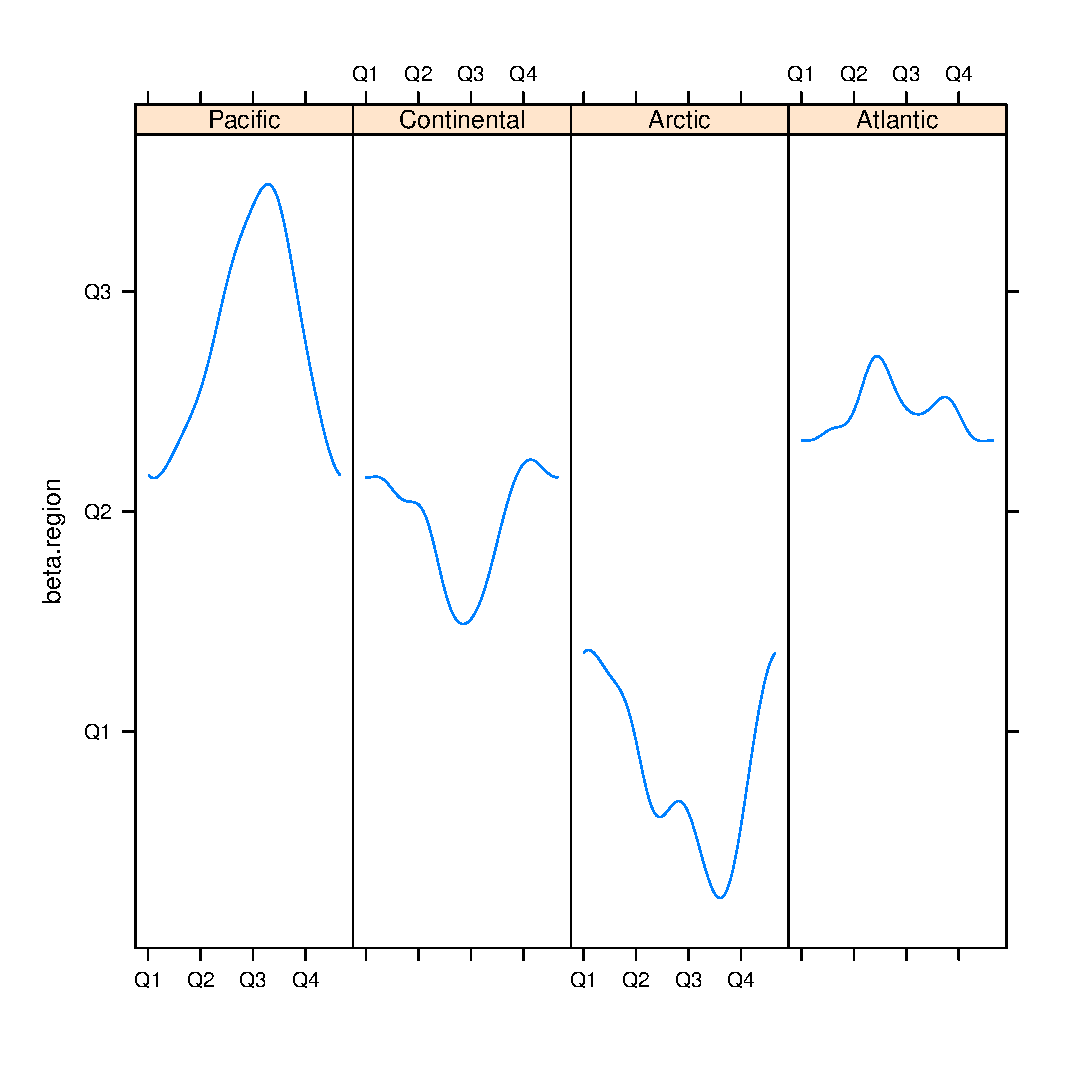
\includegraphics[height=5cm, width=9cm]{figs/tempregionbeta2}

Ramsay, Hooker, Graves (2009, Fig. 10.1)

\end{frame}

%%%%%%%%%%%%%%% fRegress.fdPar:  Concurrent Functional Model

\begin{frame}{fRegress.fdPar:  Concurrent Functional Model}

\[ y_i(t) = \beta_0(t) + \sum x_{ij}(t) \beta_j(t) + \epsilon_i(t) \]

\texttt{(knee angle) \~\ (hip angle)}

\includegraphics[height=5cm, width=9cm]{figs/gaitregression1a}

Ramsay, Hooker and Graves (2009, Fig. 10.7)

\end{frame}

%%%%%%%%%%%%%%% fRegress.formula:  Simple fRegress Setup

\begin{frame}{fRegress.formula:  Simple fRegress Setup}
Traditional:  fRegress(y, xlist, betalist) 
\newline \newline
Formula interface: 
\begin{itemize} 
    \item model <- fRegress(y \~\ x, method='model') 
    \item model = list(y, xlist, betalist) 
\end{itemize}
Manually adjust model to get what you want.
\newline \newline
Easier than manual set up, esp. w. x factors? 

\end{frame}

%%%%%%%%%%%%%%% linmod:  Full Integration Regression

\begin{frame}{linmod:  Full Integration Regression}

%\newline \newline \newline
Ramsay, Hooker and Graves (2009)
\emph{Functional Data Analysis with R and Matlab}
(Springer, ch. 10)

\end{frame}
%%%%%%%%%%%%%%% pda.fd:  Estimating a Differential Equation

\begin{frame}{pda.fd:  Estimating a Differential Equation}

%\newline \newline \newline
Ramsay, Hooker and Graves (2009)
\emph{Functional Data Analysis with R and Matlab}
(Springer, ch. 11)

\end{frame}
%%%%%%%%%%%%%%% Closing Remarks
\begin{frame}{Closing Remarks}

\end{frame}

%%%%%%%%%%%%%%% References
\begin{frame}{References}

%Software:   Ramsay, Wickham, Graves and Hooker (2009)
%\emph{fda: Functional Data Analysis. R package}, version 2.1.2
%(www.functionaldata.org)

%How to:  Ramsay, Hooker and Graves (2009)
%\emph{Functional Data Analysis with R and Matlab}
%(Springer, ch. 11)

%Theory:  Ramsay and Silverman (2005)
%\emph{Functional Data Analysis}, 2nd ed.
%(Springer)

\end{frame}

\end{document}
